\subsection*{Algemeen}
Het team van Project SUNRISE heeft deze week samen gewerkt aan een overzichtelijk systeem dat vervolgens per subgroep uitgewerkt kan worden. Een overzicht hiervan kan gevonden worden in figuur \ref{fig:algemeen_overzicht}.\\

\begin{figure}[htbp]
\centering
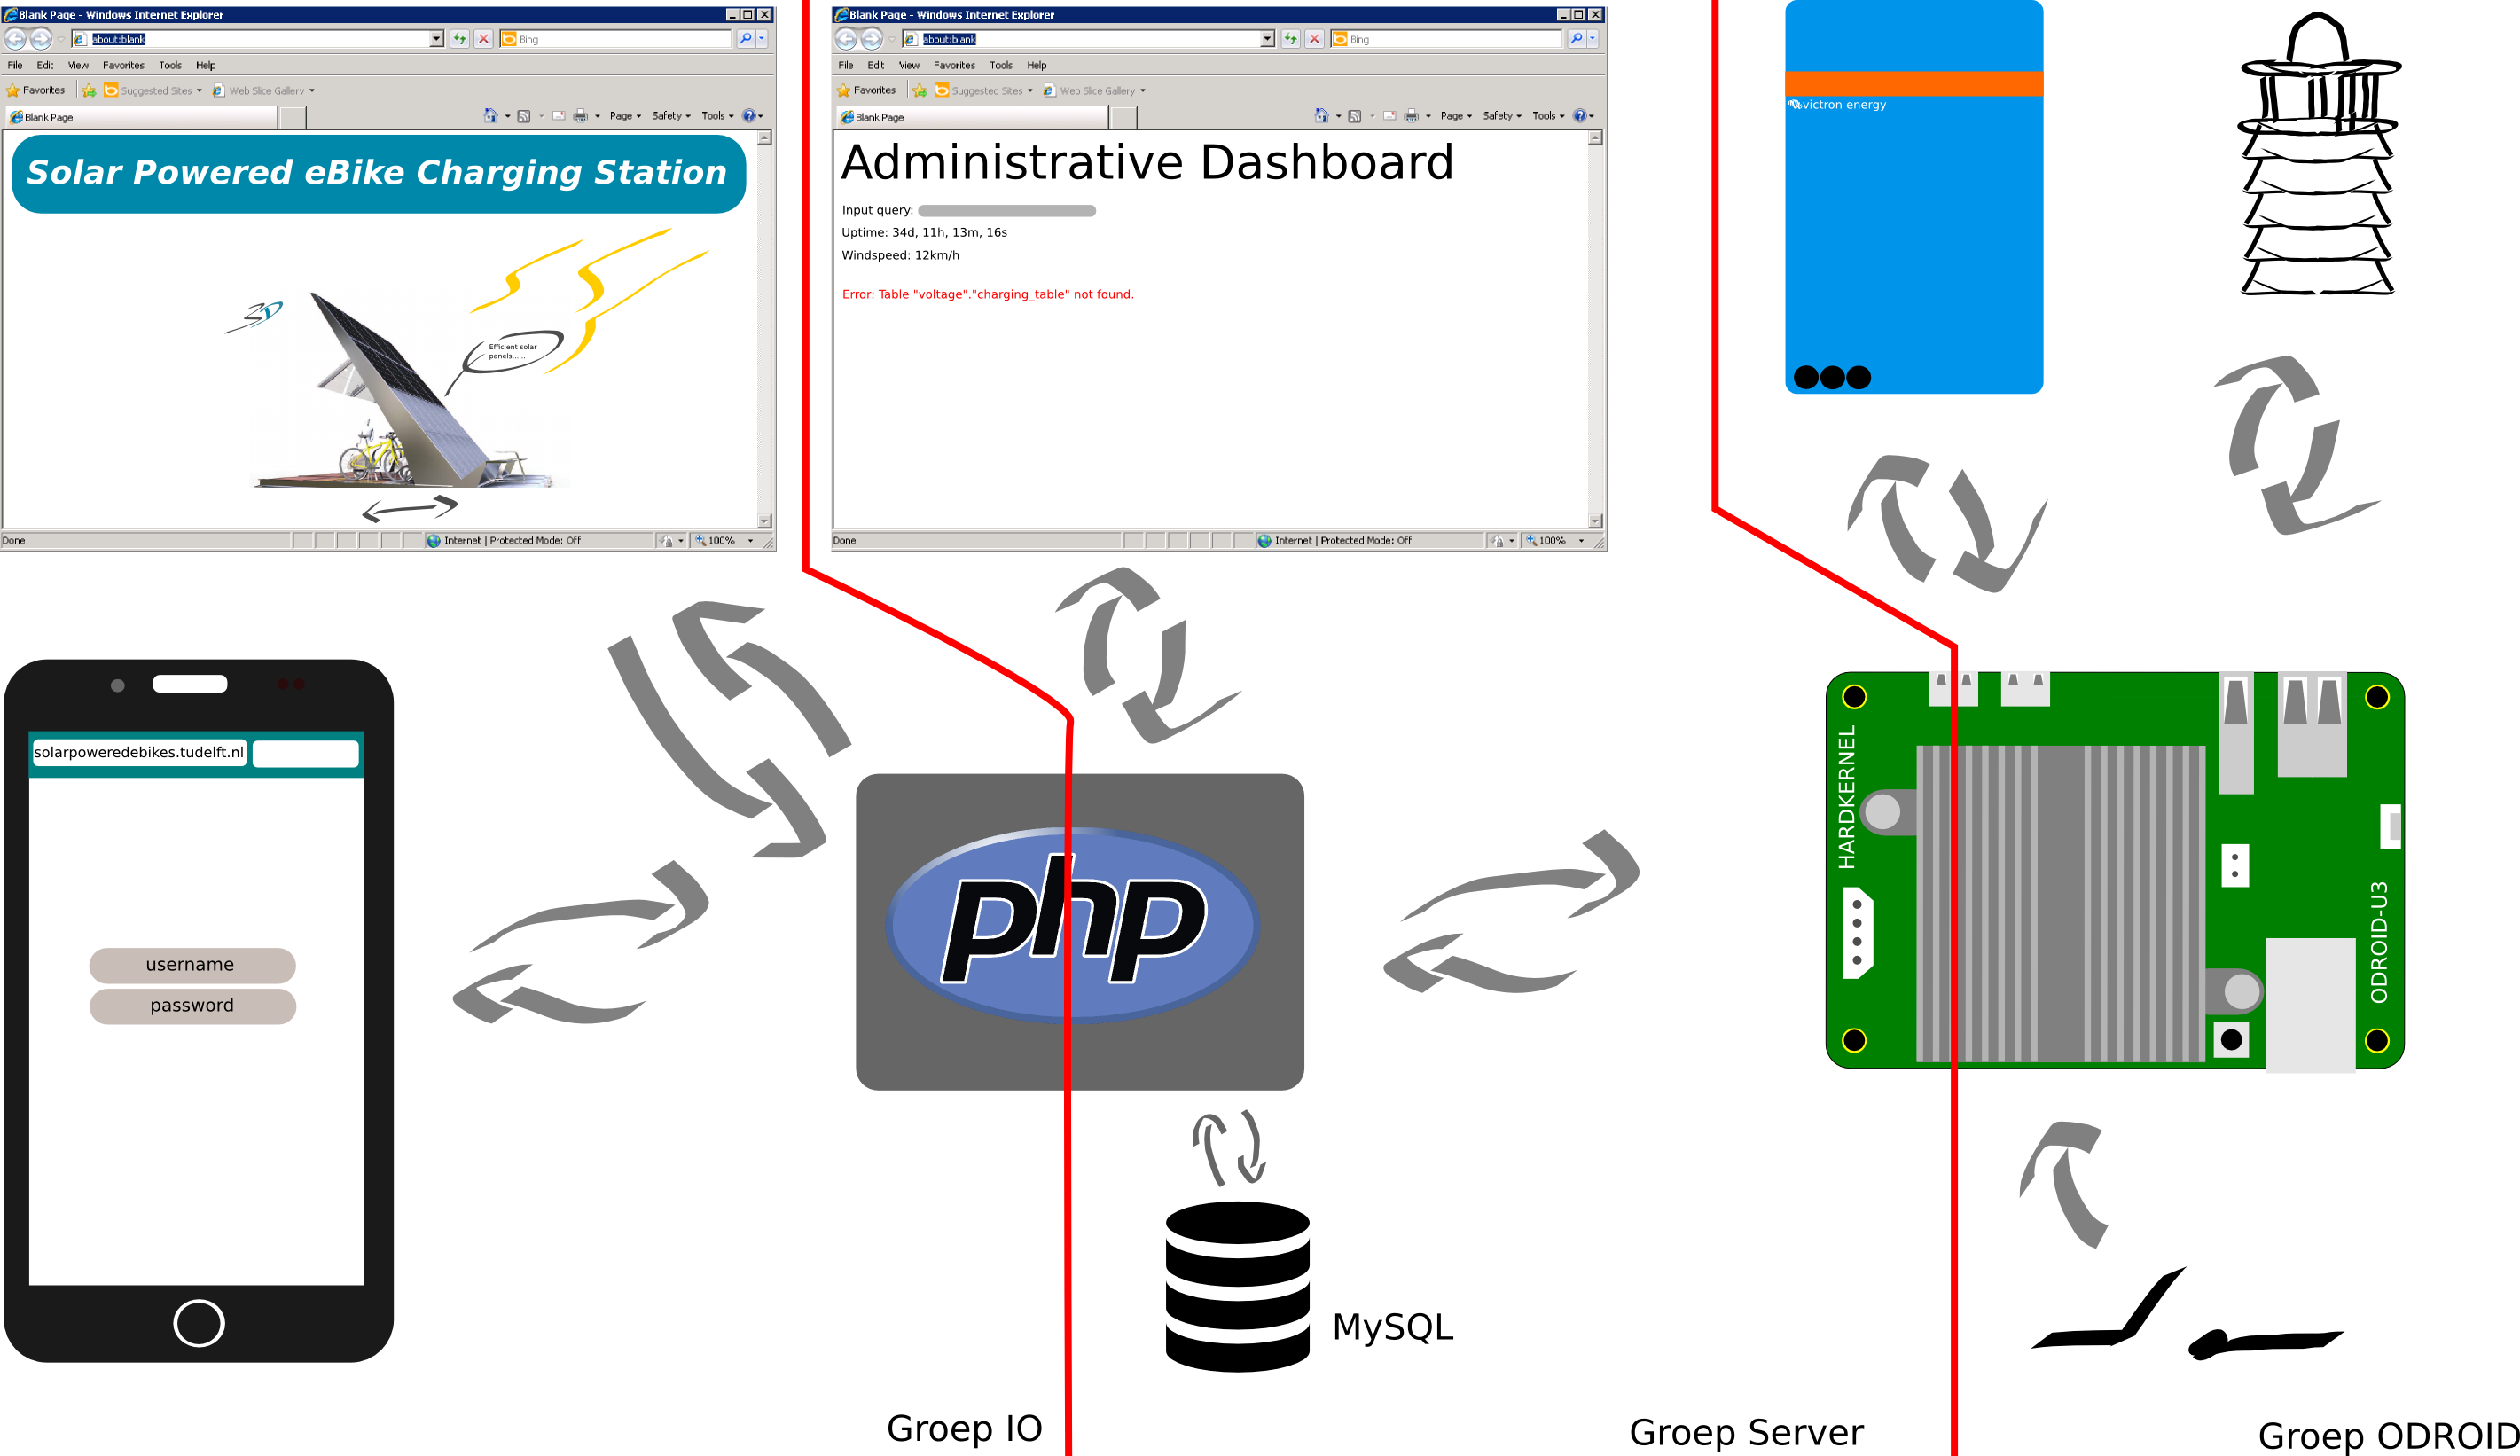
\includegraphics[width=1\textwidth]{project_overview.png}
\caption{Algemeen overzicht voor Project SUNRISE, verdeeld per groep}\label{fig:algemeen_overzicht}
\end{figure}

Bovendien is er gewerkt aan een plan van aanpak. Hierin staan bijvoorbeeld beschreven welke tussenresultaten er zijn, hoe aan de kwaliteitseisen wordt voldaan en een algemene planning.\\

Er is verder nog een naam bedacht waar de groep onder zal gaan werken: Project SUNRISE. SUNRISE staat voor "Smart Unified Networking Rig for an Integrated Solar E-bike charger".